% ***********************************************************
% ******************* PHYSICS HEADER ************************
% ***********************************************************
% Version 2.Nacho.1
\documentclass[11pt]{article} 
\usepackage{amsmath} % AMS Math Package
\usepackage{amsthm} % Theorem Formatting
\usepackage{amssymb}	% Math symbols such as \mathbb
\usepackage{graphicx} % Allows for eps images
\usepackage{multicol} % Allows for multiple columns
\usepackage[dvips,letterpaper,margin=0.75in,bottom=0.5in]{geometry}
 % Sets margins and page size
\makeatletter % Need for anything that contains an @ command 
\renewcommand{\maketitle} % Redefine maketitle to conserve space
{ \begingroup \vskip 10pt \begin{center} \large {\bf \@title}
	\vskip 10pt \large \@author \hskip 20pt \@date \end{center}
  \vskip 10pt \endgroup \setcounter{footnote}{0} }
\makeatother % End of region containing @ commands
\renewcommand{\labelenumi}{(\alph{enumi})} % Use letters for enumerate
% \DeclareMathOperator{\Sample}{Sample}
\let\vaccent=\v % rename builtin command \v{} to \vaccent{}
\renewcommand{\v}[1]{\ensuremath{\mathbf{#1}}} % for vectors
\newcommand{\gv}[1]{\ensuremath{\mbox{\boldmath$ #1 $}}} 
% for vectors of Greek letters
\newcommand{\uv}[1]{\ensuremath{\mathbf{\hat{#1}}}} % for unit vector
\newcommand{\abs}[1]{\left| #1 \right|} % for absolute value
\newcommand{\avg}[1]{\left< #1 \right>} % for average
\let\underdot=\d % rename builtin command \d{} to \underdot{}
\newcommand{\der}[2]{\frac{d #1}{d #2}} % for derivatives
\newcommand{\dder}[2]{\frac{d^2 #1}{d #2^2}} % for double derivatives
\newcommand{\dnder}[3]{\frac{d^{#3} #1}{d #2^{#3}}} % para derivadas n-esimas
\newcommand{\dpar}[2]{\frac{\partial #1}{\partial #2}}
\newcommand{\ddpar}[2]{\frac{\partial^2 #1}{\partial #2^2}} % for double partial derivatives
\newcommand{\dnpar}[3]{\frac{\partial^{#3} #1}{\partial #2^{#3}}}% para derivadas parciales n-esimas
\newcommand{\dparc}[3]{\left( \frac{\partial #1}{\partial #2}
 \right)_{#3}} % for thermodynamic partial derivatives
\newcommand{\ket}[1]{\left| #1 \right>} % for Dirac bras
\newcommand{\bra}[1]{\left< #1 \right|} % for Dirac kets
\newcommand{\braket}[2]{\left< #1 \vphantom{#2} \right|
 \left. #2 \vphantom{#1} \right>} % for Dirac brackets
\newcommand{\matrixel}[3]{\left< #1 \vphantom{#2#3} \right|
 #2 \left| #3 \vphantom{#1#2} \right>} % for Dirac matrix elements
\newcommand{\grad}[1]{\gv{\nabla} #1} % for gradient
\let\divsymb=\div % rename builtin command \div to \divsymb
\renewcommand{\div}[1]{\gv{\nabla} \cdot #1} % for divergence
\newcommand{\curl}[1]{\gv{\nabla} \times #1} % for curl
\newcommand{\ssum}[2]{\sum_{#1}^{#2}}
\newcommand{\pprod}[2]{\prod_{#1}^{#2}}
\let\baraccent=\= % rename builtin command \= to \baraccent
\renewcommand{\=}[1]{\stackrel{#1}{=}} % for putting numbers above =
\newtheorem{prop}{Proposition}
\newtheorem{thm}{Theorem}[section]
\newtheorem{lem}[thm]{Lemma}
\theoremstyle{definition}
\newtheorem{dfn}{Definition}
\theoremstyle{remark}
\newtheorem*{rmk}{Remark}

% ***********************************************************
% ********************** END HEADER *************************
% ***********************************************************


\begin{document}
\begin{titlepage}
\newcommand{\HRule}{\rule{\linewidth}{0.5mm}}
\center 
 
\textsc{\LARGE UNIVERSIDAD NACIONAL AUT\'ONOMA DE M\'EXICO}\\[1.5cm] 
\textsc{\Large Facultad de Ciencias}\\[0.5cm] 
\textsc{\large Laboratorio de electr\'onica}\\[0.5cm] 
\HRule \\[0.4cm]
{ \huge \bfseries Pr\'actica IV: Filtros}\\[0.4cm]
\HRule \\[1.5cm]
\begin{minipage}{0.4\textwidth}
\begin{flushleft} \large
\emph{Alumno:}\\
Ignacio \textsc{Loaiza}
\end{flushleft}
\end{minipage}
~
\begin{minipage}{0.4\textwidth}
\begin{flushright} \large
\emph{Profesor} \\
Dr. Jos\'e\ Manuel \textsc{Alvarado Reyes}
\end{flushright}
\end{minipage}\\[3cm]
{\large 7 de Octubre de 2014}\\[0.5cm]
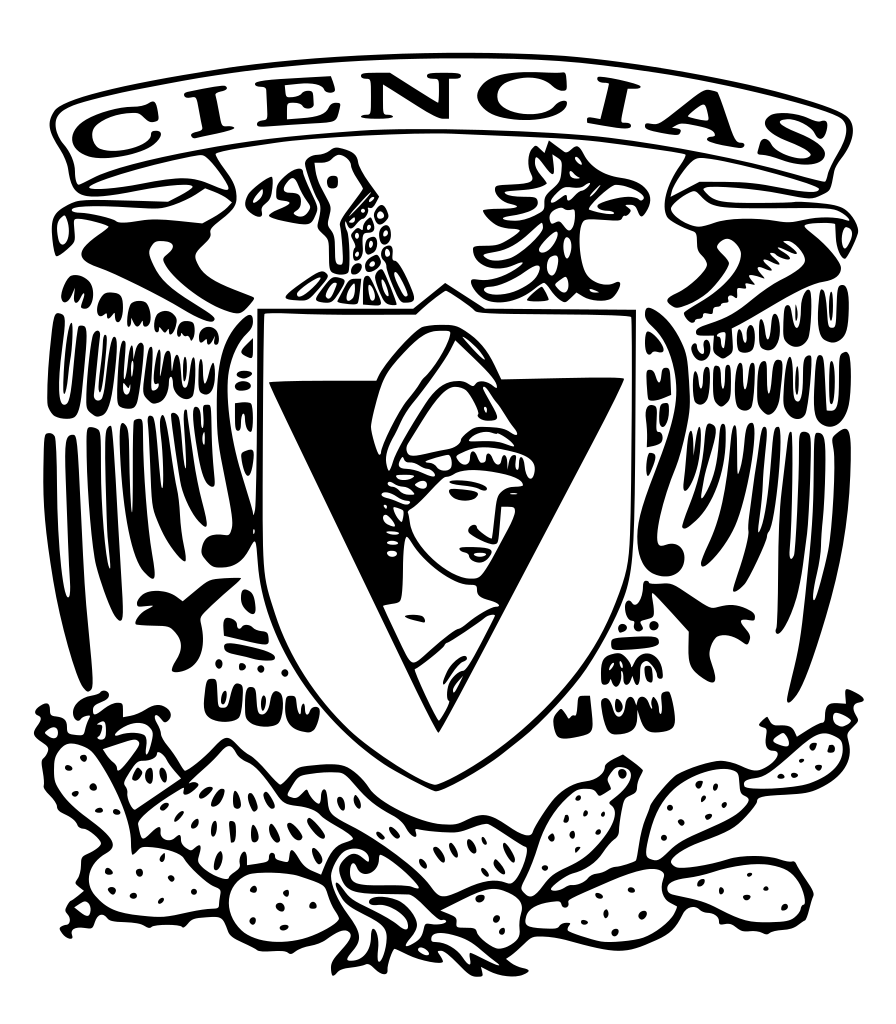
\includegraphics[width=6cm]{/home/nacho/Escuela/ciencias.png}\\[1cm]
\vfill
\end{titlepage}
\section{Resumen}
En esta pr\'actica se estudiaron los filtros pasa bajos, pasa altos, pasa bandas y de resonancia (sean filtros RC y RLC). Se observ\'o\ c\'omo camb\'ia el comportamiento de corte en los filtros cuando se var\'ian los valores de los componentes, as\'i\ como las limitantes de los filtros.

\section{Introducci\'on}
En muchas ocasiones se puede tener un voltaje alternativo con frecuencias no deseadas. Al estudiar c\'omo funcionan los filtros as\'i\ como las limitantes de estos, se puede trabajar mejor con cualquier voltaje que se tenga, aprendiendo a manipularlo de forma que podamos trabajar con el voltaje que queramos, en vez del voltaje que nos llega. Cabe destacar que los filtros son utilzados en los radios, lo cual nos muestra uno de los muchos usos que tienen, resaltando la importancia de aprender a utilizarlos.

\section{Marco te\'orico}
Los filtros son circuitos electr\'onicos con un voltaje de entrada y uno de salida. Al introducir un voltaje en el filtro, en funci\'on de la frecuencia de este se obtiene el mismo voltaje con alguna atenuaci\'on (la cual puede ser nula) a la salida. Existen varios tipos de filtros, y por lo general se caracterizan por una frecuencia de corte. La frecuencia de corte es aquella frecuencia para la cual el voltaje de salida es $V_S=\frac{1}{\sqrt{2}}V_E\approx 0.707V_E$, d\'onde $V_E$ es el voltaje de entrada. Como se ver\'a\ m\'as adelante, existen filtros que se caracterizan por varias frecuencias de corte.
\subsection*{Filtro pasa bajas}
El filtro pasa bajas, como su nombre lo indica, es un filtro que s\'olo deja pasar a las bajas frecuencias, y est\'a\ compuesto por un circuito como el que se muestra a continuaci\'on:
\begin{center}
\includegraphics[width=10cm]{bajas.png}
\end{center}
\begin{center}
Figura 1: Esquema de filtro pasa bajas.
\end{center}
La frecuencia de corte del filtro pasa bajas est\'a\ dada por:
\begin{equation}
f_c=\frac{1}{2\pi RC}
\end{equation}
D\'onde $R$ es la resistencia y $C$ la capacitancia. Se tiene entonces que el ancho de banda de un filtro pasa bajas est\'a\ dado por:
\begin{equation}
BW=\Delta f=f_c-0=f_c
\end{equation}
La curva de ganancia del voltaje en funci\'on de la frecuencia se ve entonces como:
\begin{center}
\includegraphics[width=10cm]{bajascomp.png}
\end{center}
\begin{center}
Figura 2: Ganancia del voltaje de filtro pasa bajas en funci\'on de la frecuencia de entrada.
\end{center}

\subsection*{Filtro pasa altas}
El filtro pasa altas s\'olo deja pasar a las altas frecuencias, y est\'a\ compuesto de la siguiente forma:
\begin{center}
\includegraphics[width=10cm]{altas.png}
\end{center}
\begin{center}
Figura 3: Esquema de un filtro pasa altas.
\end{center}
La frecuencia de corte de este filtro est\'a\ dada de la misma forma que para el filtro pasa bajas:
\begin{equation}
f_c=\frac{1}{2\pi RC}
\end{equation}
Y su ancho de banda estar\'ia entonces dado por:
\begin{equation}
BW=\Delta f=\infty-f_c
\end{equation}
\begin{center}
\includegraphics[width=10cm]{altascomp.png}
\end{center}
\begin{center}
Figura 4: Ganancia del voltaje de filtro pasa altas en funci\'on de la frecuencia de entrada.
\end{center}

\subsection*{Filtro pasa bandas}
El filtro pasa bandas est\'a\ compuesto por un filtro pasa altas/bajas conectado a la salida de un filtro pasa bajas/altas. Este s\'olo deja pasar frecuencias que se encuentran en un intervalo entre las dos frecuencias de corte (es importante notar que la frecuencia de corte del filtro pasa bajas debe de ser menor a la frecuencia de corte del filtro pasa altas).
El ancho de banda de este filtro est\'a\ entonces dado por:
\begin{equation}
BW=\Delta f=f_{altas}-f_{bajas}
\end{equation}

\subsection*{Filtro de resonancia}
El filtro resonante s\'olo deja pasar frecuencias cercanas a una frecuencia de resonancia, y est\'a\ compuesto de la siguiente forma:
\begin{center}
\includegraphics[width=10cm]{resonante.png}
\end{center}
\begin{center}
Figura 5: Esquema de filtro pasa bandas
\end{center}
La frecuencia de corte para este filtro est\'a\ dada por:
\begin{equation}
f_c=\frac{1}{2\pi \sqrt{LC}}
\end{equation}

\section{Experimentaci\'on}


\subsection{Filtro pasa bajas}
\subsubsection{Materiales}
\begin{itemize}
\item Generador de funciones
\item Resistencia de $1k\Omega$
\item Capacitor de $10nF$
\item Osciloscopio
\end{itemize}

\subsubsection{M\'etodo experimental}
Se arm\'o\ el circuito del filtro pasa bajas con los componentes mencionados arriba. Utilizando la funci\'on de sweep del generador y moviendo manualmente la frecuencia de salida, se busc\'o\ cual era la frecuencia de corte y se estudi\'o\ el comportamiento de la ganancia en voltaje del filtro en funci\'on de la frecuencia.

\subsubsection{Resultados y discusi\'on}
Se obtuvo una frecuencia de corte $f_c=13kHz$. Al hacer el sweep se obtuvo el siguiente voltaje:
\begin{center}
\includegraphics[width=10cm]{bajasexp.jpg}
\end{center}
\begin{center}
Figura 6: Voltaje del sweep para filtro pasa bajas.
\end{center}
Como se puede ver en la figura, el voltaje disminuye cuando aumenta la frecuencia, lo cual concuerda con el comportamiento esperado de este filtro. La frecuencia de corte te\'orica es de $f_t=15.92kHz$. Como se puede observar, la frecuencia de corte obtenida experimentalmente est\'a\ bastante cerca de la te\'orica, lo cual nos permite verificar la vericidad de la ecuaci\'on (1). Adem\'as, el ancho de bandas obtenido fue de $10kHz$ medido desde $3kHz$, lo cual concuerda con la ecuaci\'on de ancho de banda (2) $BW=f_c$.

\subsection{Filtro pasa altas}
\subsubsection{Materiales}
\begin{itemize}
\item Generador de funciones
\item Resistencia de $1k\Omega$
\item Capacitor de $10nF$
\item Osciloscopio
\end{itemize}

\subsubsection{M\'etodo experimental}
Se repiti\'o\ el m\'etodo experimental que para el filtro pasa bajas, pero armando el circuito del filtro pasa altas. Se cambi\'o\ un poar de veces el capacitor para verificar el comportamiento de la frecuencia de corte.

\subsubsection{Resultados y discusi\'on}
Se obtuvo una frecuencia de corte $f_c=13kHz$. Al hacer el sweep se obtuvo el siguiente voltaje:
\begin{center}
\includegraphics[width=10cm]{altasexp.jpg}
\end{center}
\begin{center}
Figura 7: Voltaje del sweep para filtro pasa altas.
\end{center}
Como se puede ver en la figura, el voltaje aumenta cuando aumenta la frecuencia, lo cual concuerda con el comportamiento esperado de este filtro. La frecuencia de corte te\'orica es de $f_t=15.92kHz$. Para el capacitor de $22nF$ de obtuvo una frecuencia de corte de $7kHz$, y con el de $1nF$ se obtuvo una frecuencia de corte de $173kHz$, siendo las frecuencias te\'oricas de $7.54kHz$ y de $159.2kHz$ respectivamente. Nuevamente se logr\'o\ verificar la ecuaci\'on del filtro pasa altas, verificando el comportamiento de este circuito.

\subsection{Filtro pasa bandas}
\subsubsection{Materiales}
\begin{itemize}
\item Generador de funciones
\item Resistencias de $R_1=220\Omega,\ R_2=1k\Omega$
\item Capacitores de $C_1=1nF,\ C_2=22nF$
\item Osciloscopio
\end{itemize}

\subsubsection{M\'etodo experimental}
Se arm\'o\ el filtro pasa bajas con $R_1$ y $C_2$, y a la salida de este se le coloc\'o\ un filtro pasa altas con $R_2$ y $C_1$. Cabe notar que hay que elegir valores de tal forma que la impedancia del primer filtro sea menor a la del segundo filtro. Volvi\'o\ a hacer un sweep, obteniendo el comportamiento del filtro, las frecuencias de corte y el ancho de banda. Despu\'es de hacer esto se cambi\'o\ de lugar a los filtros y se volvi\'o\ a medir el voltaje con el sweep. 
\subsubsection{Resultados y discusi\'on}
Se obtuvieron frecuencias de corte de $712Hz$ y de $5.25kHz$ para el siguiente voltaje:
\begin{center}
\includegraphics[width=10cm]{bandasexp.jpg}
\end{center}
\begin{center}
Figura 8: Voltaje del sweep para filtro pasa bandas.
\end{center}
\begin{center}
\includegraphics[width=10cm]{bandasfft.jpg}
\end{center}
\begin{center}
Figura 9: Transformada de Fourier del sweep para filtro pasa altas.
\end{center}
Se utiliz\'o\ un voltaje de entrada de $18V_p$, y el voltaje m\'aximo a la salida del filtro es de $10V_p$. Se puede ver como el filtro s\'olo dej\'o\ pasar a una banda de la frecuencia, ya que se sumaron los efectos de los filtros al no dejar pasar las frecuencias altas ni las bajas. \\
Al cambiar de lugar los filtros pasa altas y pasa bajas, utilizando a $R_1$ y a $C_2$ para el pasa altas (los mismos valores que se utilizaron para el pasa bajas en la secci\'on anterior), y a $R_2$ y $C_1$ para el pasa bajas, se obtuvo un comportamiento id\'entico al caso anterior, nada m\'as que el voltaje m\'aximo del filtro cay\'o\ a s\'lo $5V_p$. Esto se debe a que los filtros no cortan inmediatamente todo el voltaje en la frecuencia de corte, por lo cual la curva de ganancia en voltaje en funci\'on de la frecuencia est\'a\ en el caso siguiente: \\ \\ \\ \\ \\ \\ \\ \\ \\
\begin{center}
\vspace{5cm}
\end{center}
\begin{center}
Figura 10: Atenuaci\'on adicional en la ganancia de voltaje del filtro pasa bandas.
\end{center}

\subsection{Filtro resonante}
\subsubsection{Materiales}
\begin{itemize}
\item Generador de funciones
\item Resistencia de $1k\Omega$
\item Capacitores de $6.8, 25, 100, 400 $y $1600nF$
\item Bobina de $92\mu H$ y de $1.42H$
\item Osciloscopio
\end{itemize}

\subsubsection{M\'etodo experimental}
Se arm\'o\ el circuito del filtro resonante como se ve en la Figura 5. Primero se arm\'o\ el circuito con la bobina de $1.42H$ y un capacitor de $100nF$, verificando el comportamiento del filtro. Despu\'es, se cambi\'o\ a la bobina de $92\mu H$, y se fueron cambiando los capacitores, de forma que se fu\'e\ observando c\'omo cambia no s\'olo la frecuencia de corte, sino c\'omo cambia el comportamiento de corte (sea la pendiente o la geometr\'ia del "chipote" que se forma al hacer el sweep). Cabe notar que se dej\'o\ al sweep fijo en esta parte para que la comparaci\'on de las geometr\'ias tenga sentido.


\subsubsection{Resultados y discusi\'on}
Al armar el circuito con la bobina de $1.42H$ y un capacitor de $100nF$, se obtuvo el siguiente voltaje:
\begin{center}
\includegraphics[width=10cm]{resonanteexp.jpg}
\end{center}
\begin{center}
Figura 11: Voltaje obtenido para el sweep del filtro resonante con $C=100nF$ y $L=1.42H$.
\end{center}
Se obtuvo una frecuencia de corte de $377Hz$, teniendo que la frecuencia de corte te\'orica es de $422.35Hz$, pudiendo verificar entonces el comportamiento del filtro resonante. \\
Despu\'es se cambi\'o\ entre todos los capacitores con la bobina de $92\mu H$, obteniendo la siguiente tabla:
\begin{center}
\begin{tabular}{||c|c|c|c||}
\hline
Capacitor [$nF$] & Voltaje pico [$V$] & Frecuencia de corte [$kHz$] & $\alpha$ [$ms/V$] \\ \hline
6.8 & 	17 & 	220  & 	1	 		\\ \hline
25 & 	18 & 	105 & 	2			\\ \hline
100 & 	10 & 	57 & 	6			\\ \hline
400 & 	10 & 	29 & 	4			\\ \hline
1600 & 	3.1 & 	15 & 	$\infty$		\\ \hline

\end{tabular}
\end{center}
\begin{center}
Tabla 1: Voltaje pico, frecuencia de corte y coeficiente alpha obtenidos en funci\'on de la capacitancia utilizada.
\end{center}
D\'onde, para calcular al coeficiento alpha, se vi\'o\ cual es el tiempo que le tom\'o\ al voltaje bajar $5V$ desde su m\'aximo. Se tom\'o\ entonces que $\alpha=\tau/5V$. Para el capacitor de $1600nF$, como el voltaje pico fue de $3.1V$, nunca baj\'o\ los $5V$, por lo cual se tom\'o\ al tiempo como infinito. Se puede ver como, entre m\'as peque\~no es el capacitor utilizado, m\'as disminuye el coeficiente $\alpha$ (sea que se vuelve m\'as pronunciado el "chipote" en el voltaje). Sin embargo, cuando la capacitancia aument\'o\ demasiado, el voltaje pico a la salida del filtro disminuye, por lo cual el coeficiente $\alpha$ disminuy\'o\. Se puede ver el pico que se obtuvo para el capacitor de $25nF$ en la siguiente figura:

\begin{center}
\includegraphics[width=10cm]{resonantefft.jpg}
\end{center}
\begin{center}
Figura 12: Transformada de Fourier del voltaje de la Figura 12.
\end{center}

\section{Conclusi\'on}
Adem\'as de haber visto el funcionamiento de los filtros, en esta pr\'actica se pudieron ver sus limitantes. El filtro es un circuito que nos permite filtrar frecuencias, pero se puede observar como en funci\'on de c\'omo es la frecuencia que se quiere filtrar es el filtro que se tiene que utilizar. Adem\'as, se vi\'o\ la importancia de la frecuencia de corte, y es muy importante subrayar que esta no nos indica cuando se deja de tener voltaje, sino s\'olo es una disminuci\'on del voltaje m\'aximo, lo cual claramente hay que tomar en cuenta cuando se est\'en utilizando los filtros en cualquier circuito electr\'onico. Adem\'as, gracias al estudio que se hizo en la \'utlima secci\'on de la pr\'actica, se recalca la importancia de las propiedades que puede tener un filtro adem\'as de la frecuencia de corte. 


\section{Bibliograf\'ia}
\begin{enumerate}
\item I. Loaiza, \textit{Bit\'acora de laboratorio de electr\'onica 2015-1}.
\end{enumerate}
\end{document}
